\documentclass[a4paper, 11pt]{article}
\usepackage[utf8]{inputenc}
\usepackage{vhistory}
\usepackage{amsfonts}
\usepackage{mathtools}
\usepackage{float}
\usepackage{blindtext}
\usepackage[inline]{enumitem}
\usepackage{xcolor}
\usepackage{amsmath, amssymb, lmodern}
\usepackage{array}
\usepackage{listings}
\usepackage{svg}
\usepackage{color}
\usepackage{booktabs}
\usepackage{caption}
\usepackage{varioref}
\usepackage{hyperref} 
\usepackage[ruled,vlined]{algorithm2e}
\usepackage[section]{placeins}
\usepackage{comment} % enables the use of multi-line comments (\ifx \fi) 
\usepackage{graphicx}
\usepackage{lipsum} %This package just generates Lorem Ipsum filler text. 
\usepackage{fullpage} % changes the margin
\usepackage{cleveref}
\definecolor{dkgreen}{rgb}{0,0.6,0}
\definecolor{gray}{rgb}{0.5,0.5,0.5}
\definecolor{mauve}{rgb}{0.58,0,0.82}
%Includes "References" in the table of contents
\usepackage[nottoc]{tocbibind}

\DeclareMathOperator*{\argmax}{argmax} % thin space, limits underneath in displays

\newenvironment{conditions}
{\par\vspace{\abovedisplayskip}\noindent\begin{tabular}{>{$}l<{$} @{${}={}$} l}}
	{\end{tabular}\par\vspace{\belowdisplayskip}}

\renewcommand{\lstlistingname}{Algorithm}% Listing -> Algorithm
\renewcommand{\lstlistlistingname}{List of \lstlistingname s}% List of Listings -> List of Algorithms
\crefname{listing}{algorithm}{algorithms}  
\Crefname{listing}{Algorithm}{Algorithms}
\floatname{algorithm}{Procedure}

\lstset{frame=tb,
	language=Python,
	aboveskip=3mm,
	belowskip=3mm,
	showstringspaces=false,
	columns=flexible,
	basicstyle={\small\ttfamily},
	numbers=left,
	numberstyle=\tiny\color{gray},
	keywordstyle=\color{blue},
	commentstyle=\color{dkgreen},
	stringstyle=\color{mauve},
	breaklines=true,
	breakatwhitespace=true,
	tabsize=3,
	inputencoding=latin1
}

%\setlength{\belowcaptionskip}{-10pt}
\makeatletter
\renewcommand{\paragraph}{%
	\@startsection{paragraph}{4}%
	{\z@}{1.0ex \@plus 1ex \@minus .2ex}{-1em}%
	{\normalfont\normalsize\bfseries}%
}
\makeatother

\usepackage{pgfplots}
\usepackage{tikz}
\usepackage{varwidth}
\usepgfplotslibrary{fillbetween}
\usetikzlibrary{calc,trees,positioning,arrows,chains,shapes.geometric,%
	decorations.pathreplacing,decorations.pathmorphing,shapes,%
	matrix,shapes.symbols}

\tikzstyle{object} = [rectangle, rounded corners, minimum width=3cm, minimum height=1cm,text centered, draw=white]
\tikzstyle{element} = [rectangle, rounded corners, minimum width=3cm, minimum height=1cm,text centered, draw=black]
\tikzstyle{xor} = [diamond, minimum width=1cm, minimum height=1cm, text centered, draw=black]
\tikzstyle{arrow} = [thick,->,>=stealth]

\pgfplotsset{width=\textwidth, height=\textheight*0.33,compat=newest}

\definecolor{train_color_1}{HTML}{8b402a}
\definecolor{train_color_2}{HTML}{e45e2d}
\definecolor{train_color_3}{HTML}{ef9c49}
\definecolor{train_color_4}{HTML}{fdea6f}

\definecolor{test_color_1}{HTML}{192574}
\definecolor{test_color_2}{HTML}{2e62a1}
\definecolor{test_color_3}{HTML}{43a7cb}
\definecolor{test_color_4}{HTML}{9ed5cd}

\pgfplotscreateplotcyclelist{train}{
	semithick,train_color_1\\%
	semithick,train_color_2\\%
	semithick,train_color_3\\%
	semithick,train_color_4\\%
}

\pgfplotscreateplotcyclelist{test}{
	semithick,test_color_1\\%
	semithick,test_color_2\\%
	semithick,test_color_3\\%
	semithick,test_color_4\\%
}



%\captionsetup[figure]{skip=0pt}


\begin{document}
	%Header-Make sure you update this information!!!!
	\noindent
	\large\textbf{Deep Reinforcement Learning algorithms for autonomous systems}  \\
	\normalsize Prof. Pietro Michiardi - Eurecom \hfill \textbf{Report settimana 09/09/2019}\\
	\normalsize Prof. Elena Baralis - Politecnico di Torino  \hfill Piero Macaluso
	
		\tableofcontents
	\section{Problems and solutions}
	
	\subsection{Stationary policy}
	
	During the training attempts made with the implemented algorithm, a marked difference emerged between the training and the test phases. The actions of the robot in the testing phase appeared to be slow, repetitive and, even after numerous training periods, the robot continued to behave in the same way.
	
	The first attempt was to increase the learning epochs and manipulate the size of the batch extracted at each time. This choice did not allow to obtain the desired results: the intervals between one episode and the next one raised due to the increase in the previously indicated parameters, without leading to noticeable improvements. This change would have made even future experiments impossible due to the very long time spent in training.
	
	For this reason, it was useful to proceed with a revision of the previous code used to solve positively the problem provided by the OpenAI Gym \textit{Pendulum-v0} environment. In this context, the size of the system state image presented a resolution that was much smaller than the one used in the experiment with Cozmo.
	
	The decision was, therefore, to reduce the size of the Cozmo state image from 320x240 to 64x64 pixels while maintaining a batch size of 256 samples and a proportion of 100 epochs/episodes. These changes have allowed not only to solve the problem related to the stationary policy but have drastically reduced the waiting times. This result enables us to perform experiments and to obtain plots in reduced time compared to the previous situation.
	
	\subsection{Save'n'Restore phase}
	
	The previous implementation offered a state saving phase (e.g. networks, episodes, memory) that could be started by the user who deliberately chose to suspend the experiment. This type of approach reveals a critical drawback. 
	Although the connection between Cozmo, Tablet and PC is stable, a random disconnection sometimes happens: it leads to a sudden interruption of the program with consequent deterioration of the data collected so far.
	This event risked making hours of experiments vain.
	
	In order to avoid further problems of this type, we implemented a checkpoint mechanism: the system saves the state of the experiment by creating a copy that can be useful to restart the procedure. This event triggers every X episodes. In the case of undesired interruption of the program, the lost learning episodes will be paltry this time, and the experiment can restart from the last checkpoint.
	
	\subsection{First 500 episode experiment}
	
	Thanks to the improvements applied to the algorithm, it was possible to carry out the first experiment using the track. During the experiment, promising signals have finally appeared: Cozmo seems to learn, albeit in a prolonged way. The experiments were carried out on 500 episodes for a total of about 50000 learning epochs. The experiment also exploited alpha autotuning. The plot in \vref{fig:train_episode} shows that the algorithm improves and reaches a peak in episode 400: in that episode, Cozmo manages to cover about half of the circuit without crashing. A GIF image of this episode is available at: \url{https://drive.google.com/file/d/17wCT0SlqVdHrVQ4HTu3GU-Cz8Q7dFeqA/view?usp=sharing}.
	
	The trend of the averages presented in \vref{fig:reward100,fig:mean} shows an increasing average of the rewards with the passing of episodes. During the following week, we will carry out further experiments starting from this basis.
	
	\begin{figure}[H]
		\begin{tikzpicture}
		\begin{axis}[axis on top, 
		xmin=0,
		xmax=500,
		ymin=0,
		ymax=1300,
		height=\textheight*0.45,
		set layers=standard,
		cycle list name=train,
		grid=both,
		grid style={solid,gray!30!white},
		% axis lines=middle,
		xlabel=Episode,
		ylabel style={align=center}, ylabel=Reward (mm),
		%legend style={at={(0.99,0.3)},anchor=east},
		legend pos=south east,
		% extra y ticks = {90},
		% 	extra y tick style={grid=major, grid style={solid,green},y tick label style={
		% 		/pgf/number format/.cd,precision=10
		%}},
		% x label style={at={(axis description cs:0.5,0)},anchor=north},
		%y label style={at={(axis description cs:-0.1,.5)},rotate=90,anchor=south}
		]
		
		\addplot table[x=Step,y=Value, col sep=comma] {plot/SAC/cozmodriver-v0/train/episode/mean.csv};
		%\addlegendentry{Mean Reward of last 100 episode};
		\addlegendentry{Mean $\mu$};
		\addlegendentry{Area $[min, max]$};
		\addlegendentry{Area $[\mu-\sigma, \mu+\sigma]$};
		
		\end{axis}
		\end{tikzpicture}
		\caption{Total reward for each episode. The maximum value of about 1200mm is at iteration 400.}
		\label{fig:train_episode}
		
		\end{figure}
	\begin{figure}[H]
		\begin{tikzpicture}
		\begin{axis}[axis on top, 
		xmin=0,
		xmax=500,
		ymin=0,
		ymax=600,
		height=\textheight*0.40,
		set layers=standard,
		cycle list name=train,
		grid=both,
		grid style={solid,gray!30!white},
		% axis lines=middle,
		xlabel=Episode,
		ylabel style={align=center}, ylabel=Reward (mm),
		%legend style={at={(0.99,0.3)},anchor=east},
		legend pos=south east,
		% extra y ticks = {90},
		% 	extra y tick style={grid=major, grid style={solid,green},y tick label style={
		% 		/pgf/number format/.cd,precision=10
		%}},
		% x label style={at={(axis description cs:0.5,0)},anchor=north},
		%y label style={at={(axis description cs:-0.1,.5)},rotate=90,anchor=south}
		]
		
		\addplot table[x=Step,y=Value, col sep=comma] {plot/SAC/cozmodriver-v0/test/rewardMean/mean.csv};
		%\addlegendentry{Mean Reward of last 100 episode};
		\addlegendentry{Mean $\mu$};
		\addlegendentry{Area $[min, max]$};
		\addlegendentry{Area $[\mu-\sigma, \mu+\sigma]$};
		
		\end{axis}
		\end{tikzpicture}
		\caption{Mean reward of 5 episode of test. The maximum value is at iteration 380.}
		\label{fig:test_episode}
		
	\end{figure}

\begin{figure}[H]
	\begin{tikzpicture}
	\begin{axis}[axis on top, 
	xmin=0,
	xmax=500,
	ymin=100,
	ymax=300,
	height=\textheight*0.45,
	set layers=standard,
	cycle list name=train,
	grid=both,
	grid style={solid,gray!30!white},
	% axis lines=middle,
	xlabel=Episode,
	ylabel style={align=center}, ylabel=Reward (mm),
	%legend style={at={(0.99,0.3)},anchor=east},
	legend pos=south east,
	% extra y ticks = {90},
	% 	extra y tick style={grid=major, grid style={solid,green},y tick label style={
	% 		/pgf/number format/.cd,precision=10
	%}},
	% x label style={at={(axis description cs:0.5,0)},anchor=north},
	%y label style={at={(axis description cs:-0.1,.5)},rotate=90,anchor=south}
	]
	
	\addplot table[x=Step,y=Value, col sep=comma] {plot/SAC/cozmodriver-v0/train/meanLast100/mean.csv};
	%\addlegendentry{Mean Reward of last 100 episode};
	\addlegendentry{Mean $\mu$};
	\addlegendentry{Area $[min, max]$};
	\addlegendentry{Area $[\mu-\sigma, \mu+\sigma]$};
	
	\end{axis}
	\end{tikzpicture}
	\caption{Mean reward of the last 100 episodes.}
	\label{fig:reward100}
	
\end{figure}

\begin{figure}[H]
	\begin{tikzpicture}
	\begin{axis}[axis on top, 
	xmin=0,
	xmax=500,
	ymin=100,
	ymax=300,
	height=\textheight*0.45,
	set layers=standard,
	cycle list name=train,
	grid=both,
	grid style={solid,gray!30!white},
	% axis lines=middle,
	xlabel=Episode,
	ylabel style={align=center}, ylabel=Reward (mm),
	%legend style={at={(0.99,0.3)},anchor=east},
	legend pos=south east,
	% extra y ticks = {90},
	% 	extra y tick style={grid=major, grid style={solid,green},y tick label style={
	% 		/pgf/number format/.cd,precision=10
	%}},
	% x label style={at={(axis description cs:0.5,0)},anchor=north},
	%y label style={at={(axis description cs:-0.1,.5)},rotate=90,anchor=south}
	]
	
	\addplot table[x=Step,y=Value, col sep=comma] {plot/SAC/cozmodriver-v0/train/mean/mean.csv};
	%\addlegendentry{Mean Reward of last 100 episode};
	\addlegendentry{Mean $\mu$};
	\addlegendentry{Area $[min, max]$};
	\addlegendentry{Area $[\mu-\sigma, \mu+\sigma]$};
	
	\end{axis}
	\end{tikzpicture}
	\caption{Mean reward of all episodes.}
	\label{fig:mean}
	
\end{figure}

\begin{figure}[H]
	\begin{tikzpicture}
	\begin{axis}[axis on top, 
	height=\textheight*0.45,
	set layers=standard,
	cycle list name=train,
	grid=both,
	grid style={solid,gray!30!white},
	% axis lines=middle,
	xlabel=Epoch,
	ylabel style={align=center}, ylabel=Value,
	%legend style={at={(0.99,0.3)},anchor=east},
	legend pos=south east,
	% extra y ticks = {90},
	% 	extra y tick style={grid=major, grid style={solid,green},y tick label style={
	% 		/pgf/number format/.cd,precision=10
	%}},
	% x label style={at={(axis description cs:0.5,0)},anchor=north},
	%y label style={at={(axis description cs:-0.1,.5)},rotate=90,anchor=south}
	]
	
	\addplot table[x=Step,y=Value, col sep=comma] {plot/SAC/cozmodriver-v0/train/alpha/mean.csv};
	%\addlegendentry{Mean Reward of last 100 episode};
	\addlegendentry{Mean $\mu$};
	\addlegendentry{Area $[min, max]$};
	\addlegendentry{Area $[\mu-\sigma, \mu+\sigma]$};
	
	\end{axis}
	\end{tikzpicture}
	\caption{Value of alpha during the training}
	\label{fig:alpha}
	
\end{figure}

\begin{figure}[H]
	\begin{tikzpicture}
	\begin{axis}[axis on top, 
	height=\textheight*0.45,
	set layers=standard,
	cycle list name=train,
	grid=both,
	grid style={solid,gray!30!white},
	% axis lines=middle,
	xlabel=Epoch,
	ylabel style={align=center}, ylabel=Value,
	%legend style={at={(0.99,0.3)},anchor=east},
	legend pos=south east,
	% extra y ticks = {90},
	% 	extra y tick style={grid=major, grid style={solid,green},y tick label style={
	% 		/pgf/number format/.cd,precision=10
	%}},
	% x label style={at={(axis description cs:0.5,0)},anchor=north},
	%y label style={at={(axis description cs:-0.1,.5)},rotate=90,anchor=south}
	]
	
	\addplot table[x=Step,y=Value, col sep=comma] {plot/SAC/cozmodriver-v0/train/critic1/mean.csv};
	%\addlegendentry{Mean Reward of last 100 episode};
	\addlegendentry{Mean $\mu$};
	\addlegendentry{Area $[min, max]$};
	\addlegendentry{Area $[\mu-\sigma, \mu+\sigma]$};
	
	\end{axis}
	\end{tikzpicture}
	\caption{Critic 1 Loss}
	\label{fig:critic1}
	
\end{figure}

\begin{figure}[H]
	\begin{tikzpicture}
	\begin{axis}[axis on top, 
	height=\textheight*0.45,
	set layers=standard,
	cycle list name=train,
	grid=both,
	grid style={solid,gray!30!white},
	% axis lines=middle,
	xlabel=Epoch,
	ylabel style={align=center}, ylabel=Value,
	%legend style={at={(0.99,0.3)},anchor=east},
	legend pos=south east,
	% extra y ticks = {90},
	% 	extra y tick style={grid=major, grid style={solid,green},y tick label style={
	% 		/pgf/number format/.cd,precision=10
	%}},
	% x label style={at={(axis description cs:0.5,0)},anchor=north},
	%y label style={at={(axis description cs:-0.1,.5)},rotate=90,anchor=south}
	]
	
	\addplot table[x=Step,y=Value, col sep=comma] {plot/SAC/cozmodriver-v0/train/critic2/mean.csv};
	%\addlegendentry{Mean Reward of last 100 episode};
	\addlegendentry{Mean $\mu$};
	\addlegendentry{Area $[min, max]$};
	\addlegendentry{Area $[\mu-\sigma, \mu+\sigma]$};
	
	\end{axis}
	\end{tikzpicture}
	\caption{Critic 2 Loss}
	\label{fig:critic2}
	
\end{figure}


\begin{figure}[H]
	\begin{tikzpicture}
	\begin{axis}[axis on top, 
	height=\textheight*0.45,
	set layers=standard,
	cycle list name=train,
	grid=both,
	grid style={solid,gray!30!white},
	% axis lines=middle,
	xlabel=Epoch,
	ylabel style={align=center}, ylabel=Value,
	%legend style={at={(0.99,0.3)},anchor=east},
	legend pos=south east,
	% extra y ticks = {90},
	% 	extra y tick style={grid=major, grid style={solid,green},y tick label style={
	% 		/pgf/number format/.cd,precision=10
	%}},
	% x label style={at={(axis description cs:0.5,0)},anchor=north},
	%y label style={at={(axis description cs:-0.1,.5)},rotate=90,anchor=south}
	]
	
	\addplot table[x=Step,y=Value, col sep=comma] {plot/SAC/cozmodriver-v0/train/entropy/mean.csv};
	%\addlegendentry{Mean Reward of last 100 episode};
	\addlegendentry{Mean $\mu$};
	\addlegendentry{Area $[min, max]$};
	\addlegendentry{Area $[\mu-\sigma, \mu+\sigma]$};
	
	\end{axis}
	\end{tikzpicture}
	\caption{Entropy target Loss}
	\label{fig:entropy}
	
\end{figure}

\begin{figure}[H]
	\begin{tikzpicture}
	\begin{axis}[axis on top, 
	height=\textheight*0.45,
	set layers=standard,
	cycle list name=train,
	grid=both,
	grid style={solid,gray!30!white},
	% axis lines=middle,
	xlabel=Epoch,
	ylabel style={align=center}, ylabel=Value,
	%legend style={at={(0.99,0.3)},anchor=east},
	legend pos=south east,
	% extra y ticks = {90},
	% 	extra y tick style={grid=major, grid style={solid,green},y tick label style={
	% 		/pgf/number format/.cd,precision=10
	%}},
	% x label style={at={(axis description cs:0.5,0)},anchor=north},
	%y label style={at={(axis description cs:-0.1,.5)},rotate=90,anchor=south}
	]
	
	\addplot table[x=Step,y=Value, col sep=comma] {plot/SAC/cozmodriver-v0/train/policy/mean.csv};
	%\addlegendentry{Mean Reward of last 100 episode};
	\addlegendentry{Mean $\mu$};
	\addlegendentry{Area $[min, max]$};
	\addlegendentry{Area $[\mu-\sigma, \mu+\sigma]$};
	
	\end{axis}
	\end{tikzpicture}
	\caption{Policy Loss}
	\label{fig:policy}
	
\end{figure}

\begin{figure}[ht!]
	\centering
	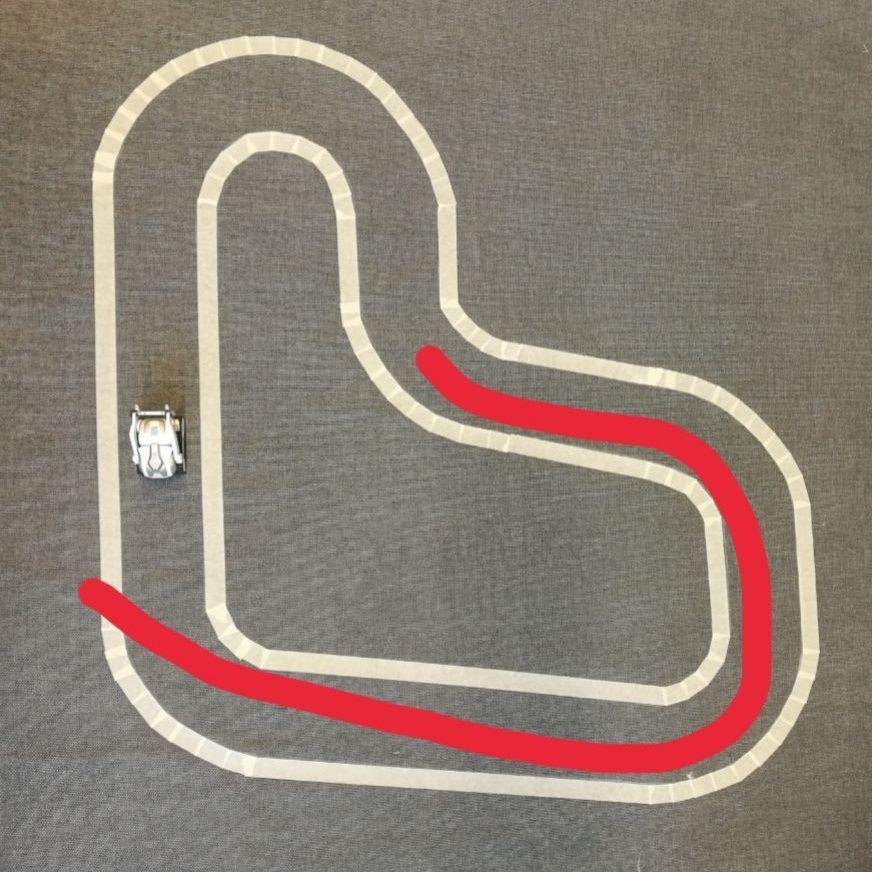
\includegraphics[height=0.4\paperwidth]{img/cozmo.jpg}
	\caption{Episode 400 of Cozmo}
	\label{fig:cozmo}
\end{figure}
	\section{Next Steps}
	 
	\subsection{Cozmo-DDPG}
	
	One crucial step for the thesis is the implementation of the DDPG algorithm for Cozmo in order to carry out a comparison between the two approaches.
	
	\subsection{Experiments}
	
	Now that the implementation allows more suitable learning timing, the next step is starting a batch of experiments using different environments (e.g. single-lane, single-line) on at least 300-500 episodes. This step is crucial to see how learning evolves and then check if the robot is learning or not.
	
	
	\newpage
	
	%\bibliographystyle{unsrt}
	%\bibliography{references}
	
\end{document}
